\hthree{Allgemein}

Für das Projektmanagement wird Github verwendet. Github bietet die Möglichkeit, einzelne Arbeitspakete zu erstellen und diese Meilensteinen und Unterprojekten Zuzuordnen. Dabei ist es möglich, dass der Status eines einzelnen Arbeitspaketes automatisch in die Spalten "To Do", "In Progress", "Review in progress", "Review approved" und "Done" verschoben wird.

\hthree{Erstellen eines Projektes}

Um ein Projekt zu erstellen, muss man zunächst ein Projekt im "Projects"-Tab (Abbildung \ref{fig:newProject}) erstellt werden.

\begin{figure}[H]
    \centering
    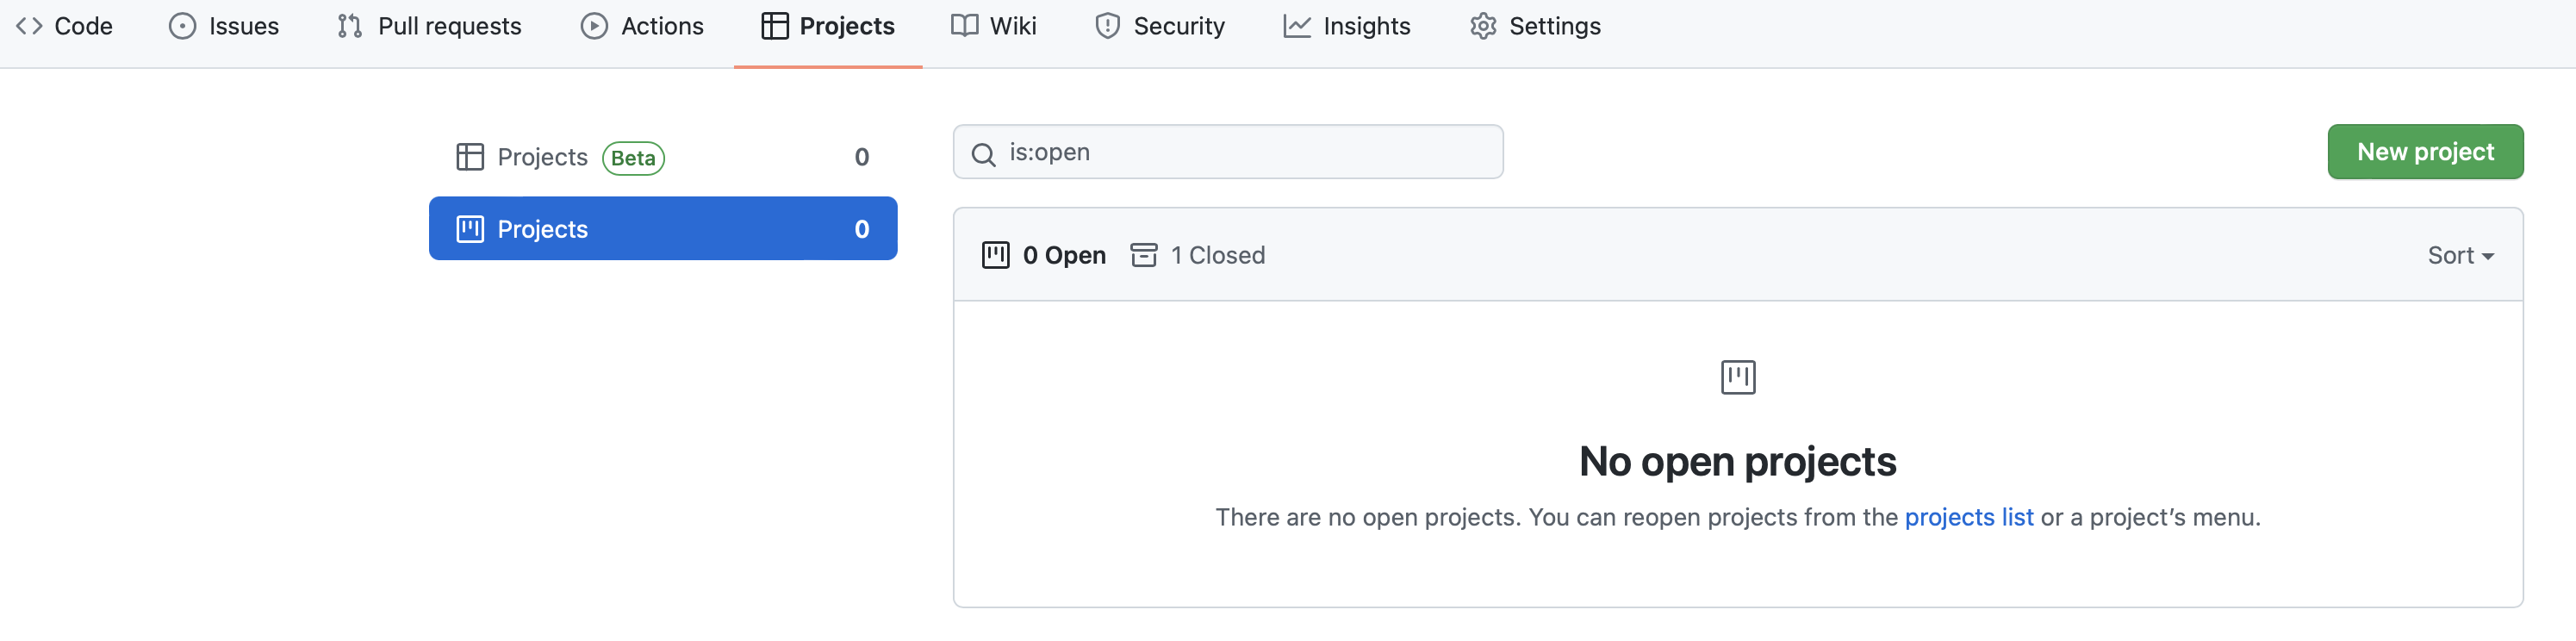
\includegraphics[width=\textwidth]{media/ProjectManagement/CreateProject.png}
    \caption{Github Projektübersicht mit "New Project" Button}
    \label{fig:newProject}
\end{figure}

Einem Projekt wird ein Name und eine Beschreibung zugewiesen. Außerdem muss das Projekt-"template" auf "Automated kanban with reviews" gesetzt werden, damit die Spalten "To Do", "In Progress", "Review in progress", "Review approved" und "Done" erstellt und die Verschiebung der Karten automatisiert wird. (Siehe Abbildung \ref{fig:enterProjectInfo})

\begin{figure}[H]
    \centering
    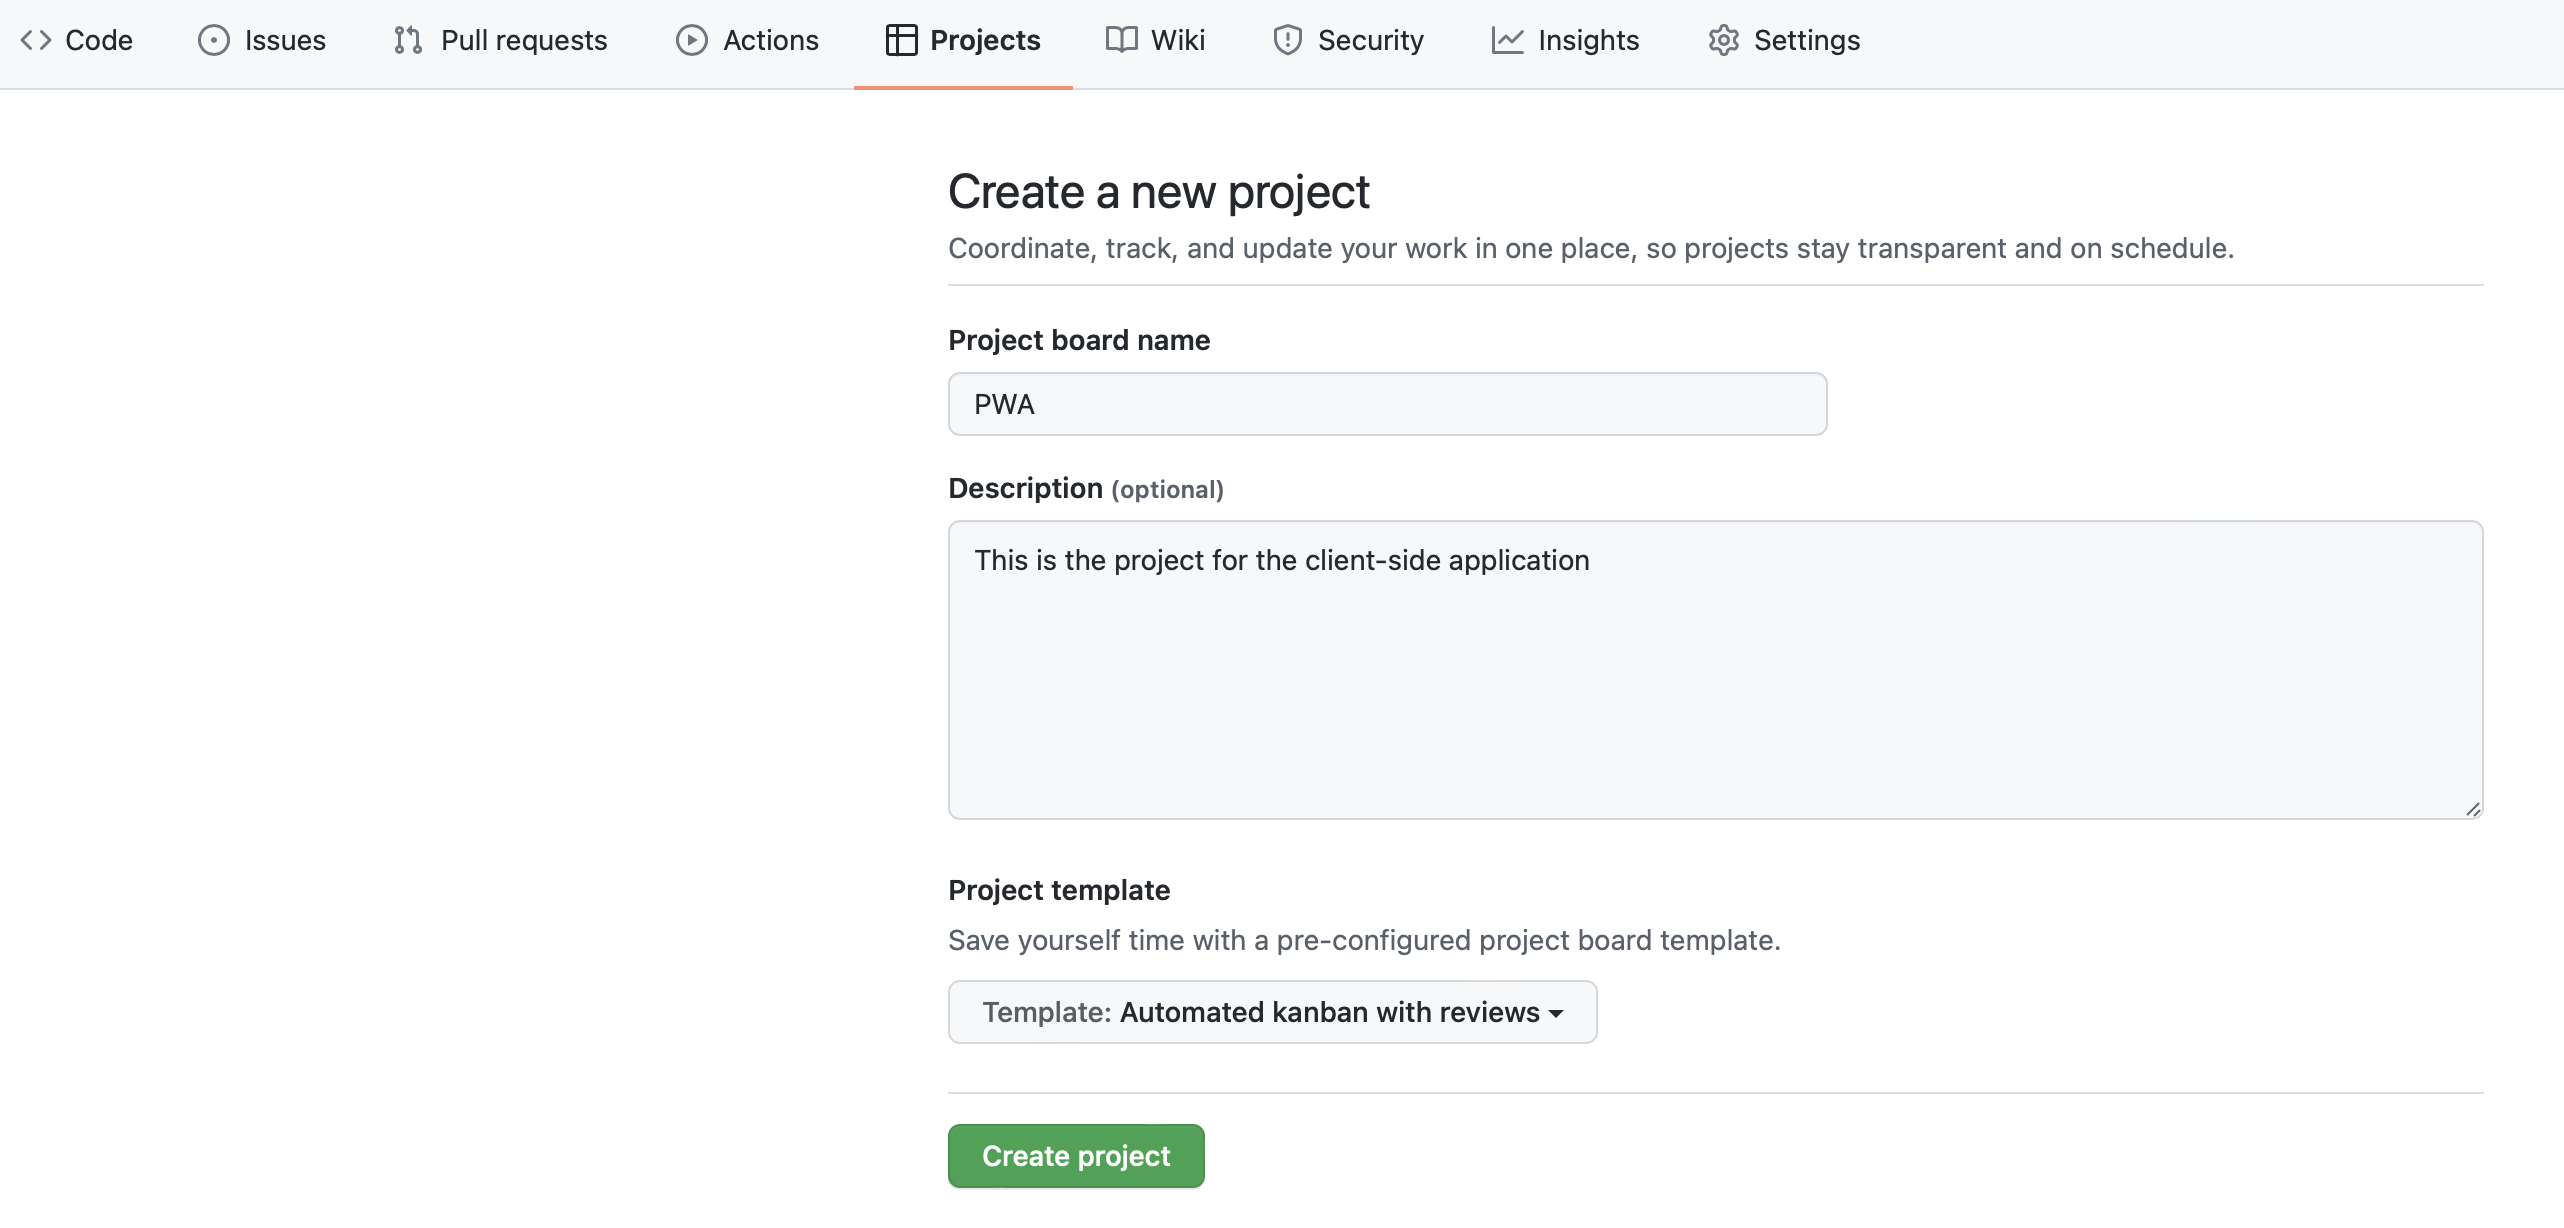
\includegraphics[width=\textwidth]{media/ProjectManagement/EnterProjectInfo.png}
    \caption{Eingabe der Projektinformationen (Demo-Bild)}
    \label{fig:enterProjectInfo}
\end{figure}

\hthree{Erstellen eines Arbeitspaketes}

Im "Issues"-Tab lassen sich Meilensteine und Label erstellen. Durch Label kann man die Art der Arbeitspakete angeben. Diese können zum Beschreibung eine neue Funktionalität oder eine Fehlerbehebung sein. Um das Arbeitspaket selbst zu erstellen, muss ein Titel vergeben werden. Außerdem werden Meilenstein, Labels und ein oder mehrere Entwickler angegeben, welche dieses Arbeitspaket bearbeiten sollen. (Siehe Abbildung \ref{fig:createIssue})

\begin{figure}[H]
    \centering
    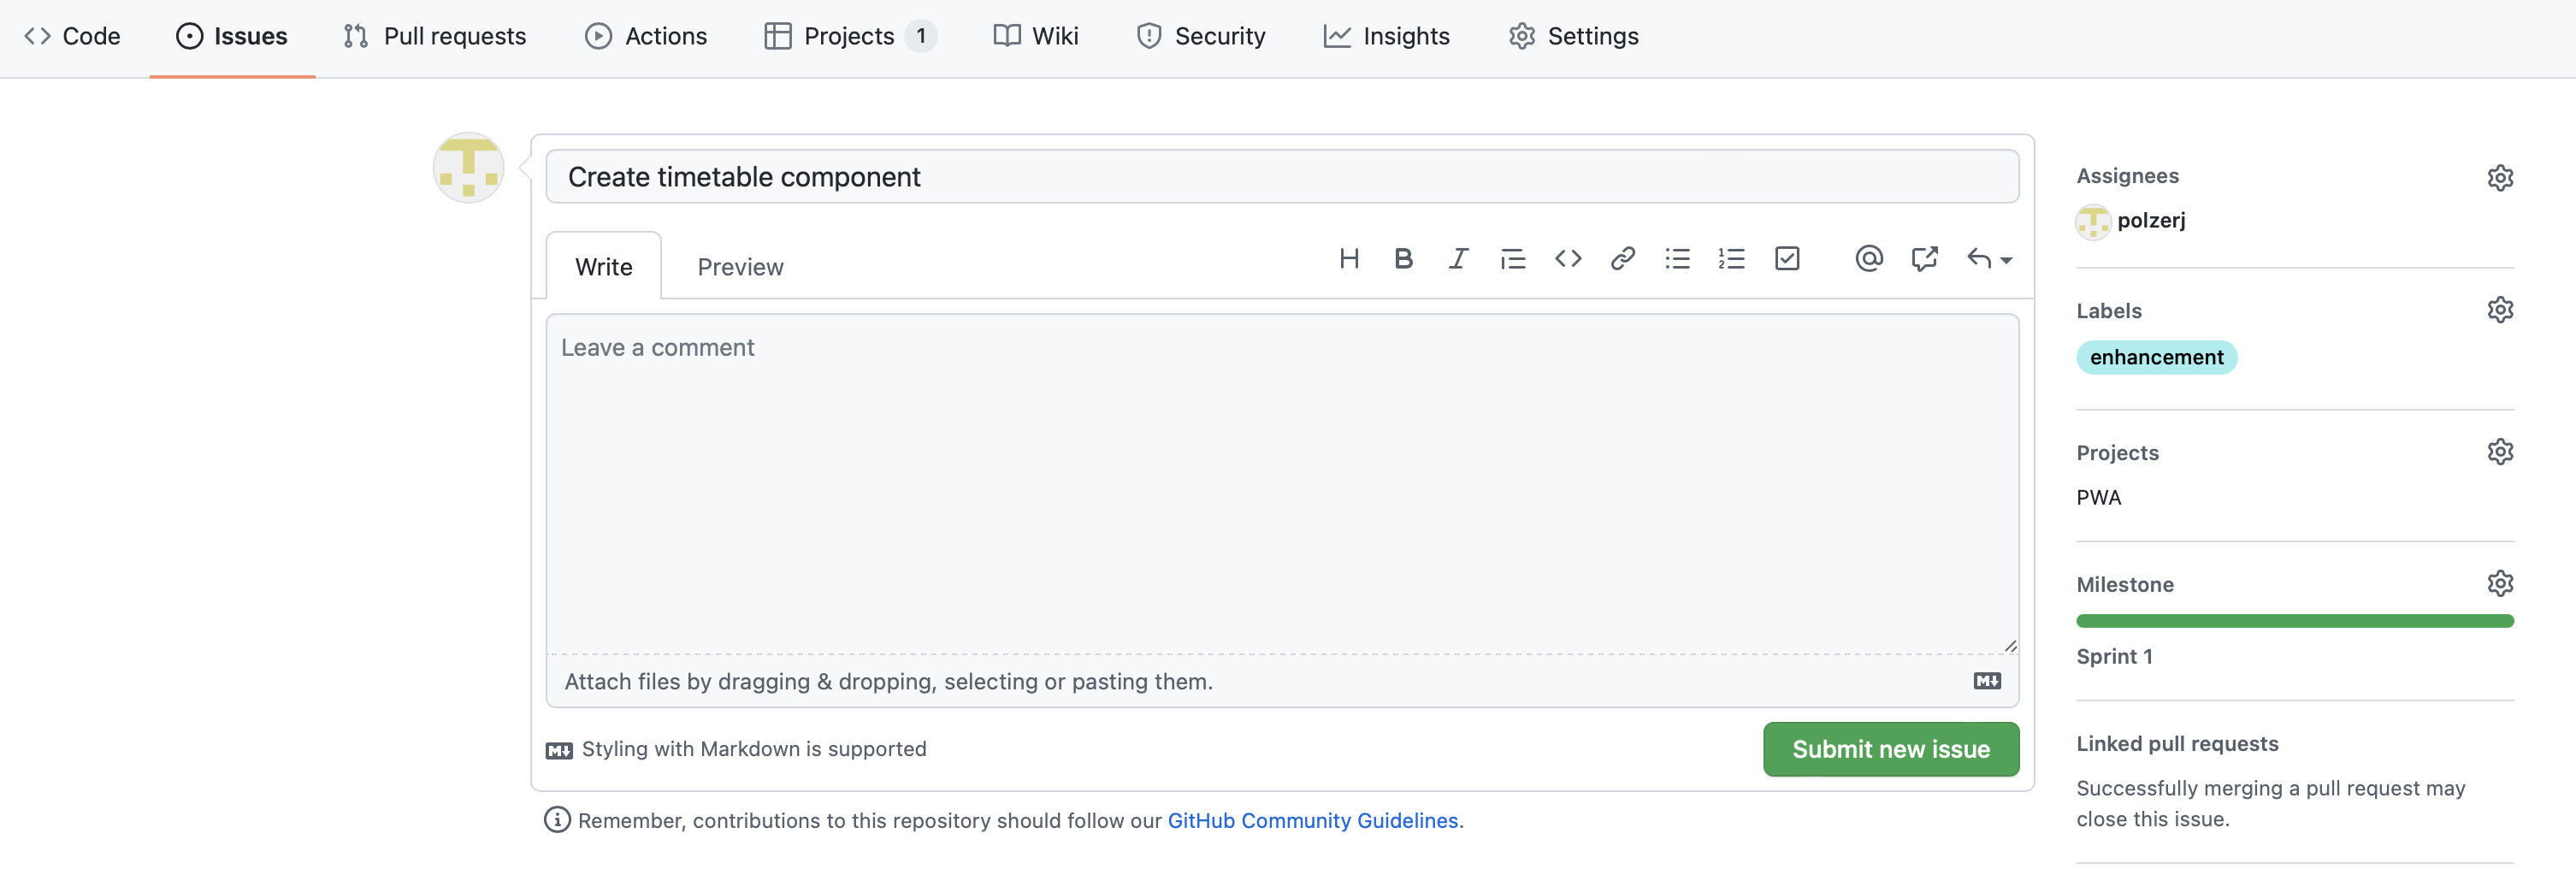
\includegraphics[width=\textwidth]{media/ProjectManagement/CreateIssue.png}
    \caption{Eingabe der Arbeitspaketinformationen (Demo-Bild)}
    \label{fig:createIssue}
\end{figure}

\hthree{Arbeiten an einem Arbeitspaket}

Für jedes Arbeitspaket wird ein eigener Branch mit dem Befehl {\ttfamily git checkout -b <Branch Namen>} erstellt. Dabei wird der Namen zusammengesetzt aus der "Issue ID" und dem "Issue"-Titel. Die "Issue ID" wird aus der Detailansicht eines "Issues" neben dem Titel entnommen. (Siehe Abbildung \ref{fig:issueInfo})  Dieser Branch kann mit dem Befehl {\ttfamily git push -u origin <Branch Namen>} auf Github hochgeladen werden. 

\begin{figure}[H]
    \centering
    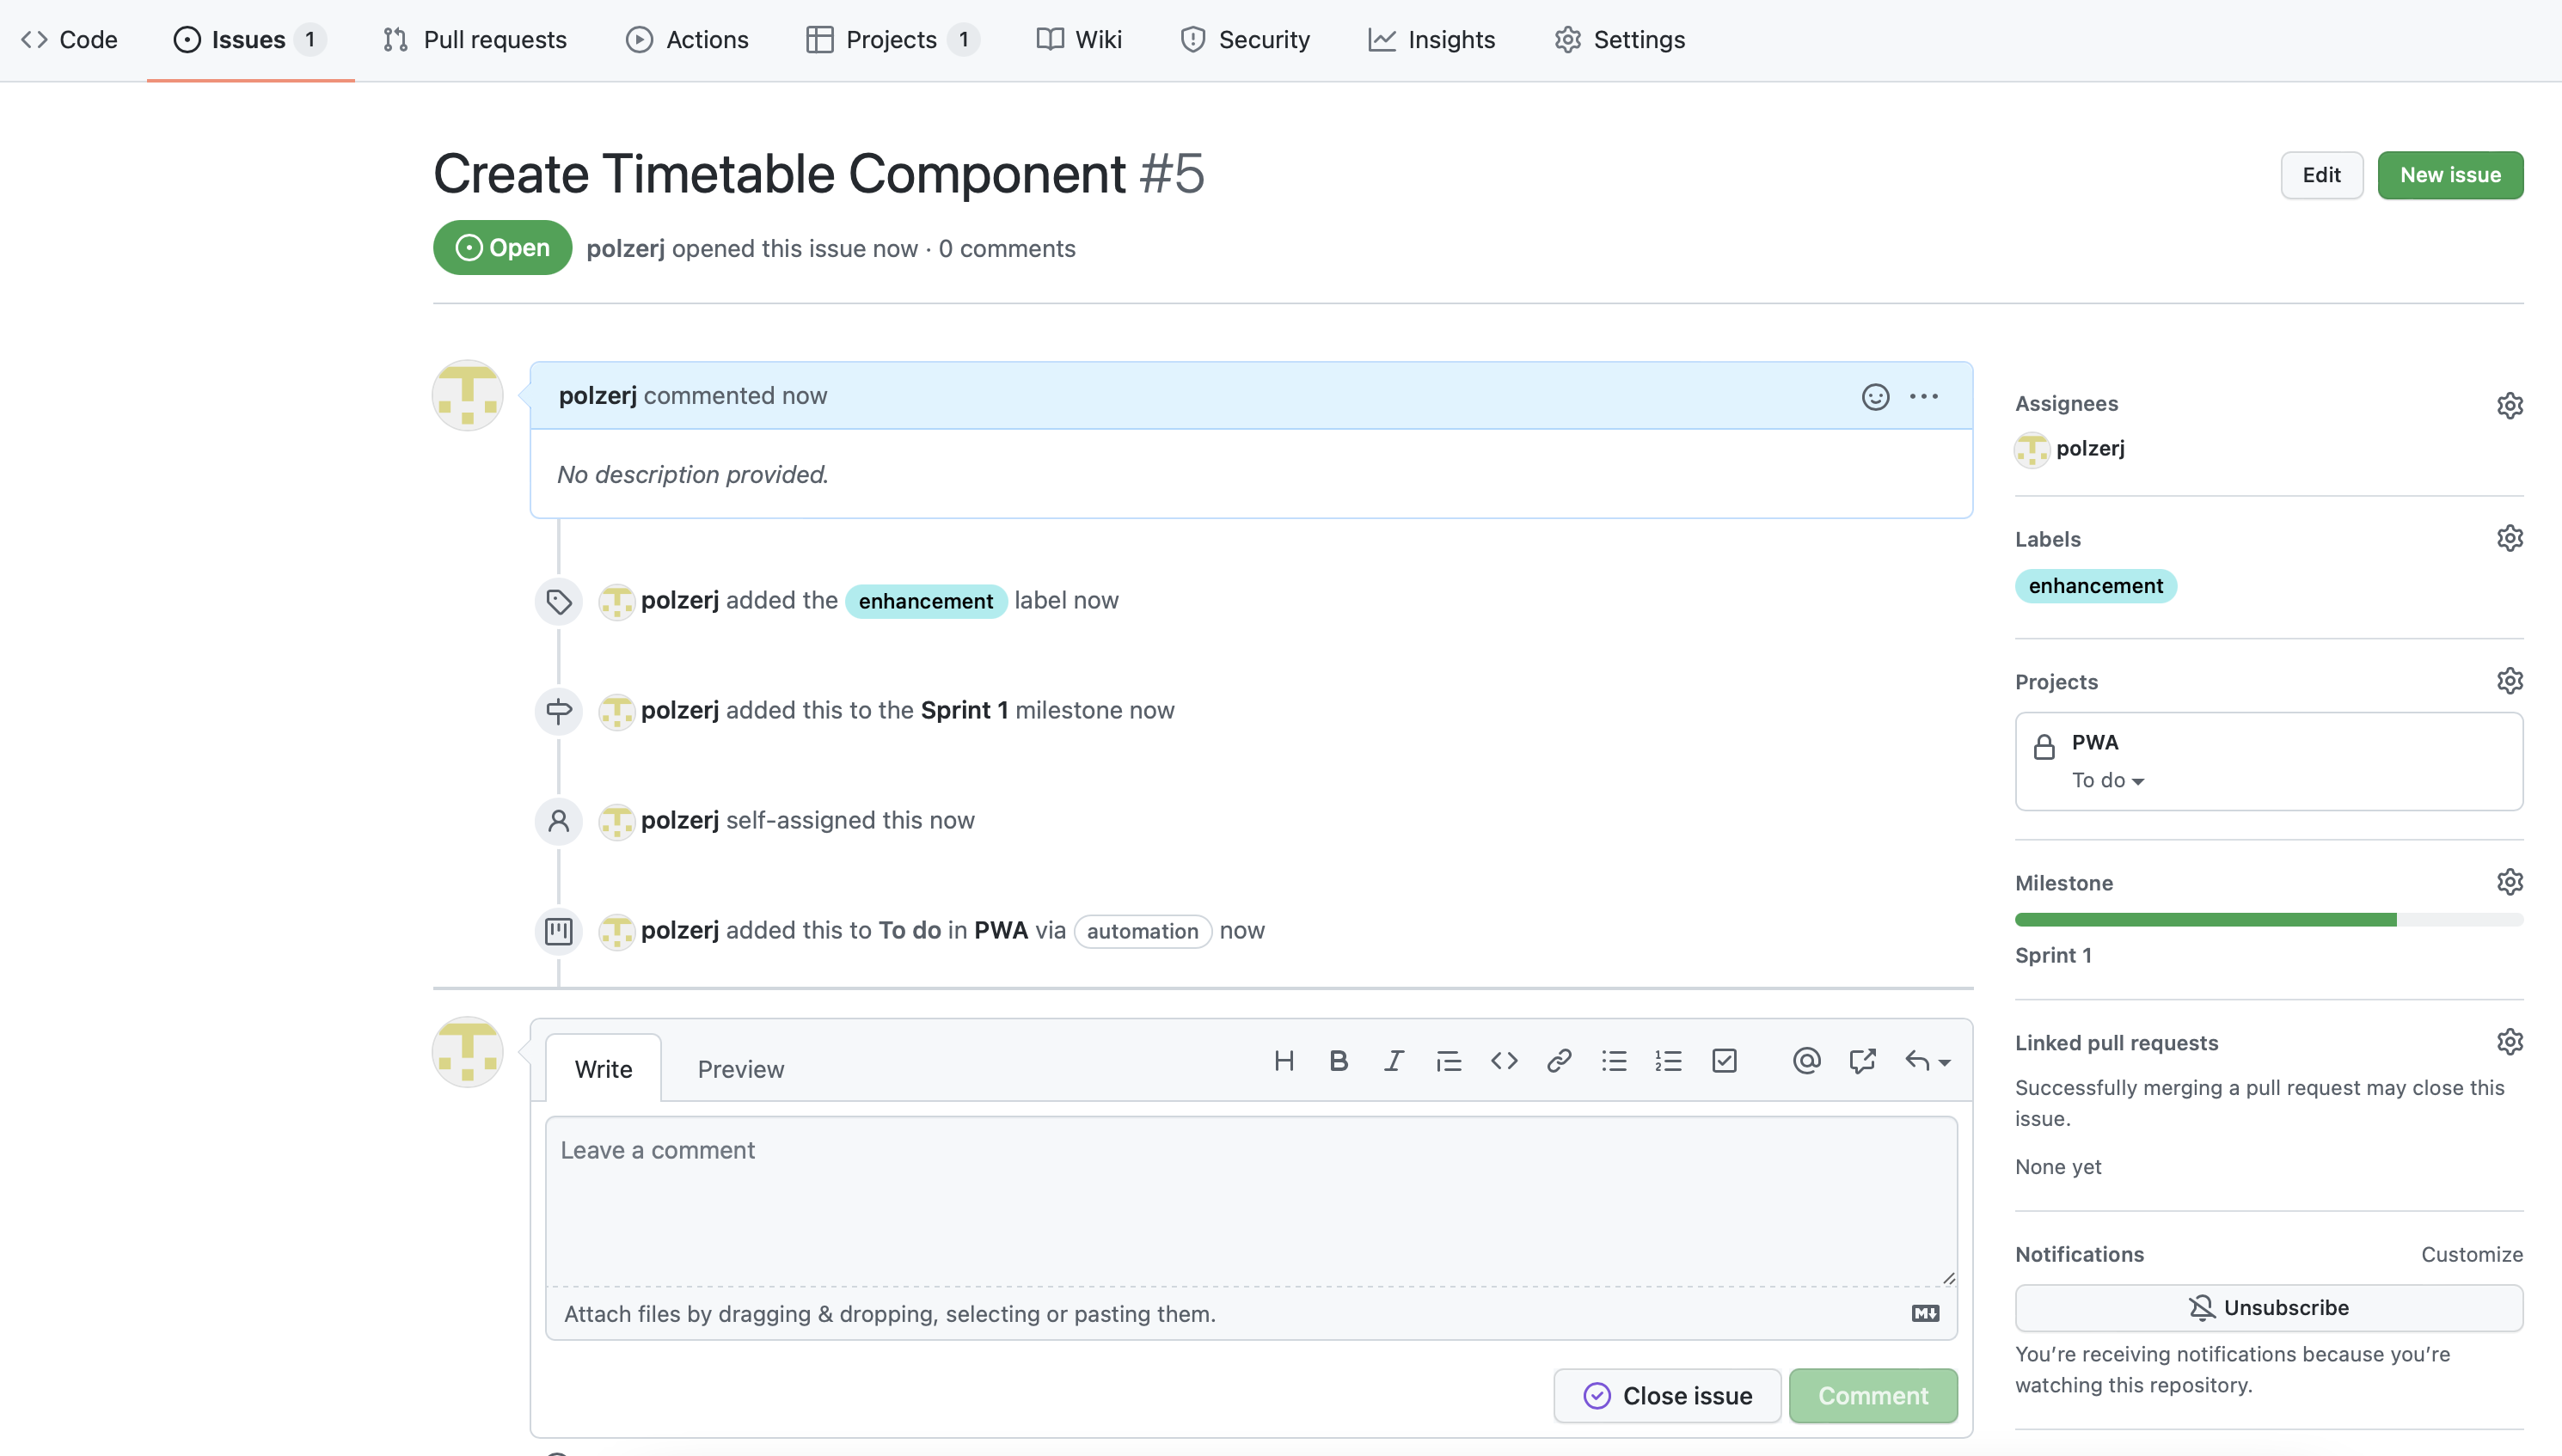
\includegraphics[width=\textwidth]{media/ProjectManagement/IssueInfo.png}
    \caption{Detailansicht "Issue" (Demo-Bild)}
    \label{fig:issueInfo}
\end{figure}

\hthree{Review und Merge}

Wenn die gesamte Funktionalität des Arbeitspakets implementiert ist, wird ein sogenannter "Pull Request" erstellt. Dies wird im "Pull Requests"-Tab gemacht. Zunächst muss ausgewählt werden, auf welchen Branch der jeweilige Arbeits-branch zusammengefügt werden soll. (Siehe Abbildung \ref{fig:createPullRequest}) Dabei wird zunächst immer auf den Branch des jeweiligen Sprints ausgewählt. Erst am Ende eines Sprints wird ein "Pull Request" von dem Branch des Sprints auf den "main"-Branch erstellt.

\begin{figure}[H]
    \centering
    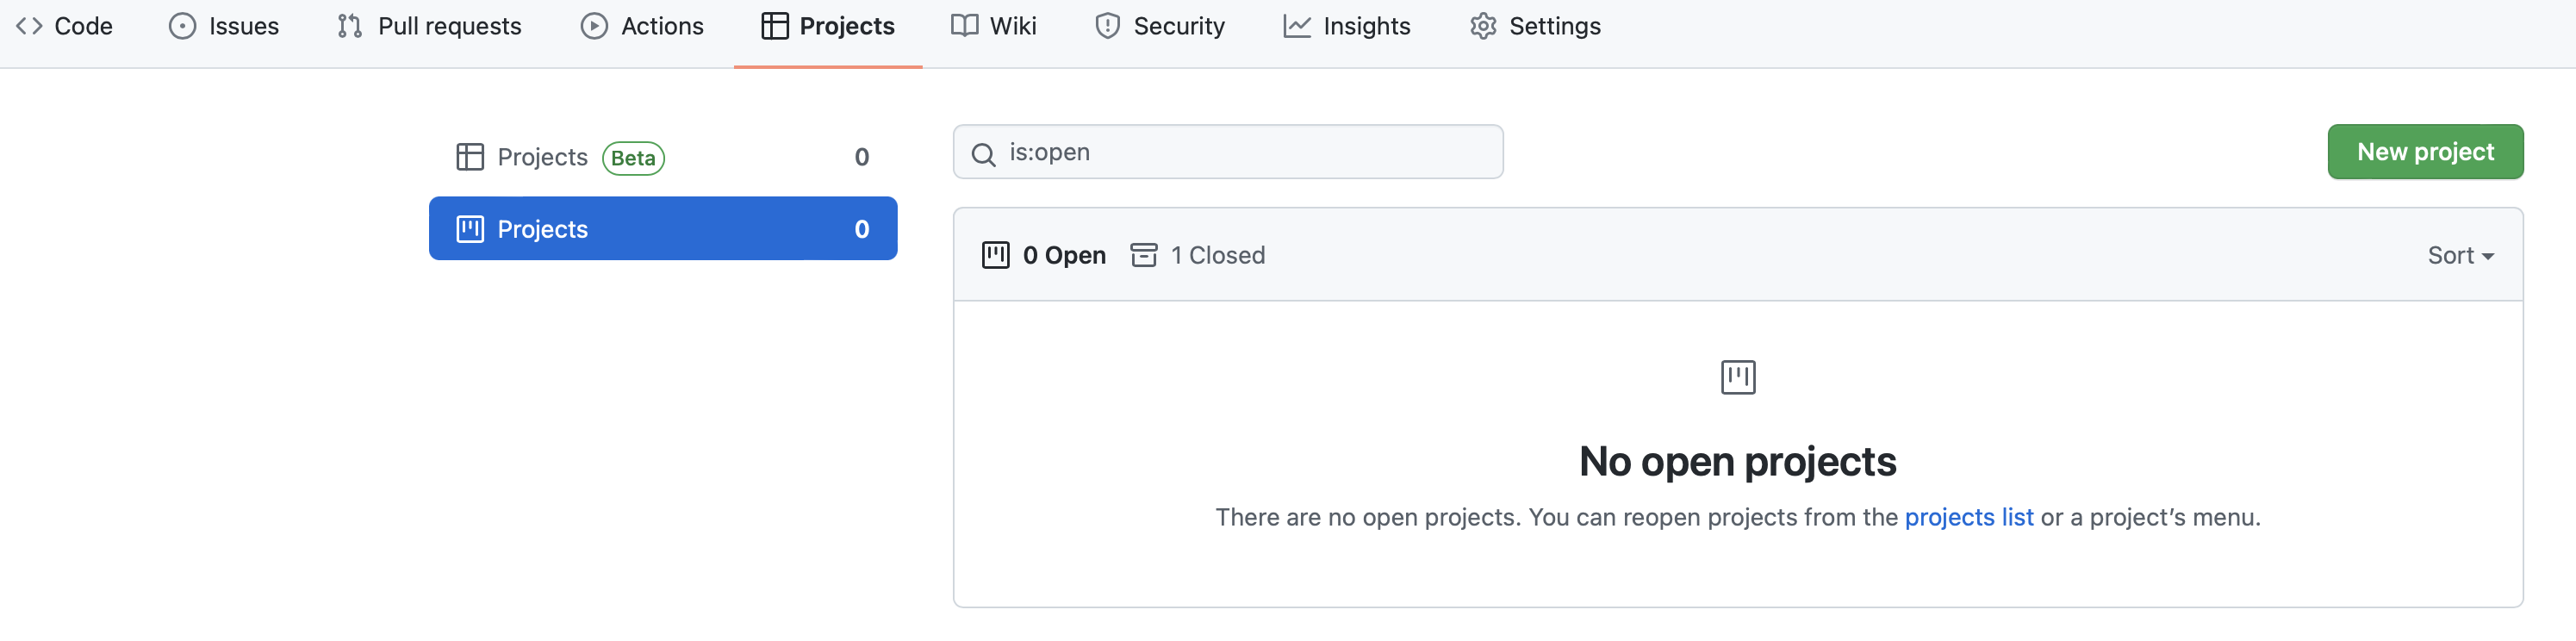
\includegraphics[width=\textwidth]{media/ProjectManagement/CreateProject.png}
    \caption{Erstellen eines "Pull Requests" (Demo-Bild)}
    \label{fig:createPullRequest}
\end{figure}

Um den "Pull Request" zu erstellen, müssen zu den im Issue schon bekannten angegebenen Feldern die Reviewer eingetragen werden. Außerdem muss in der Beschreibung des "Pull Request" "Closes \textless Issue ID\textgreater" angegeben werden. (Siehe Abbildung \ref{fig:EnterPullRequestInfo})

\begin{figure}[H]
    \centering
    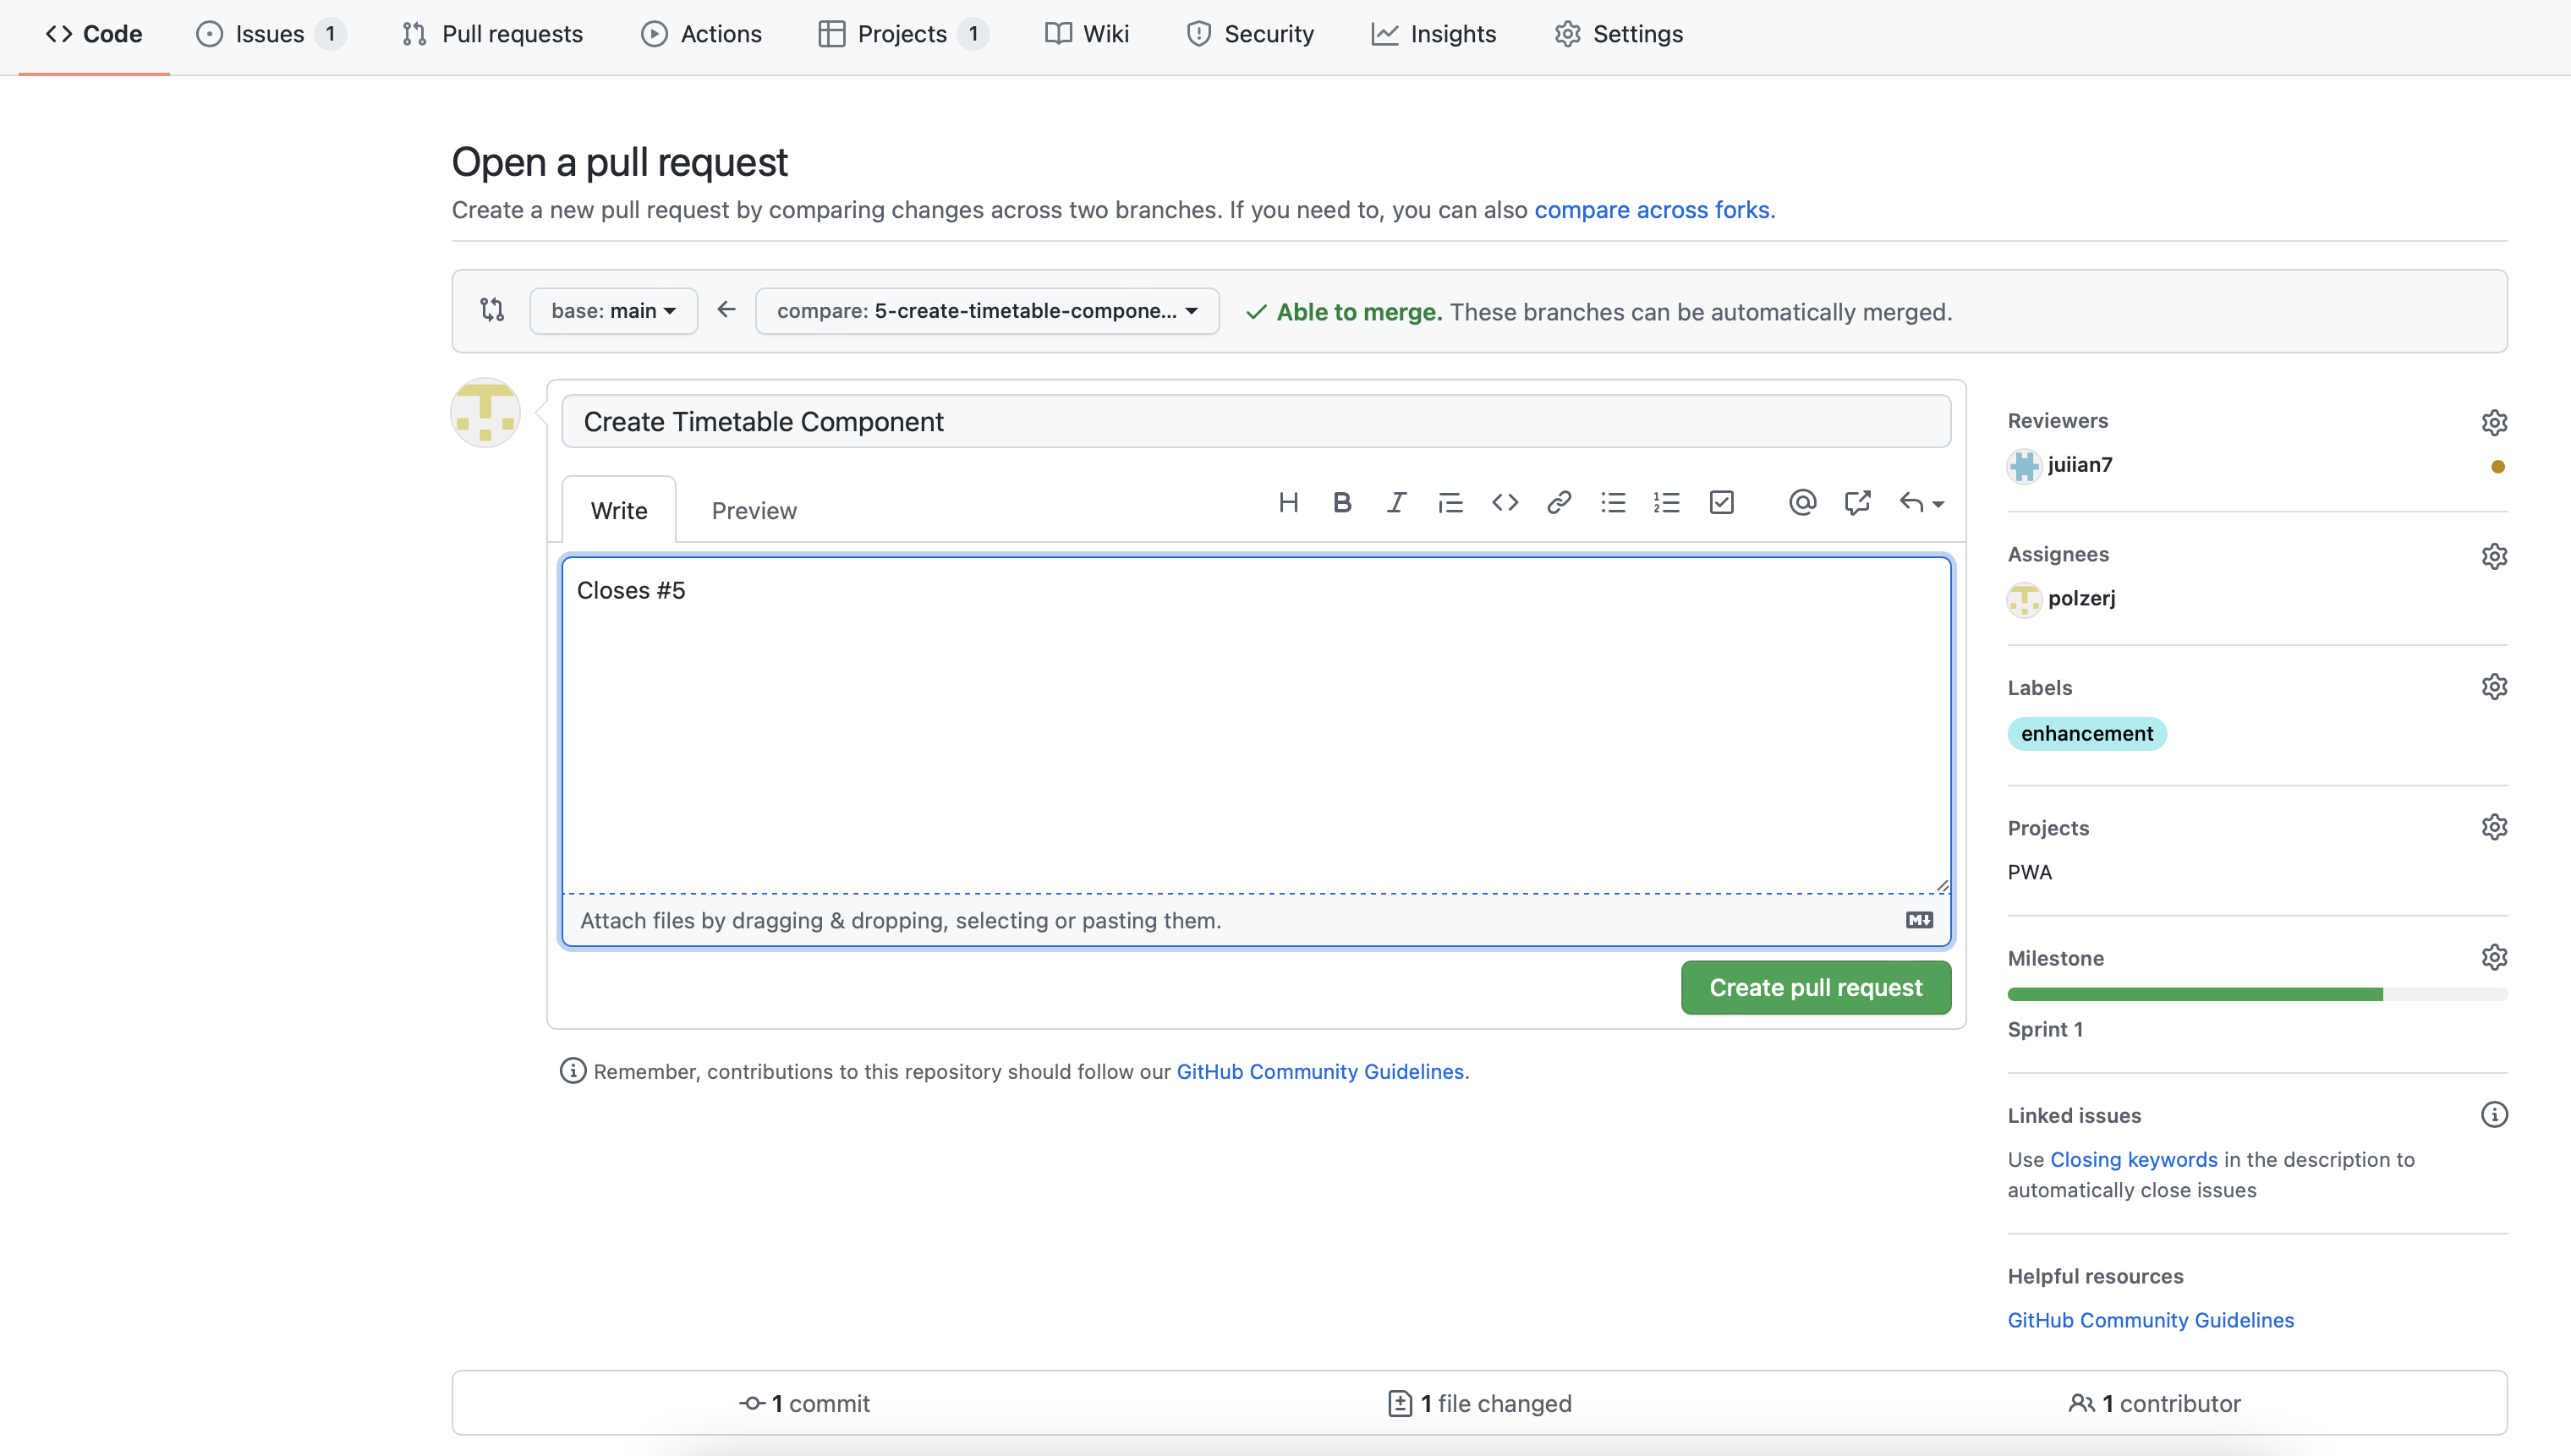
\includegraphics[width=\textwidth]{media/ProjectManagement/EnterPullInfo.png}
    \caption{Setzten der Informationen eines "Pull Requests" (Demo-Bild)}
    \label{fig:EnterPullRequestInfo}
\end{figure}

Die Reviewer können nun im "Files Changed" Tab des "Pull Requests" den Code überprüfen und daraufhin Änderungen anfordern oder des "Pull Request" freigeben. 


Wenn alle Änderungen akzeptiert werden, wird ein "Squash and Merge" durchgeführt. (Siehe Abbildung \ref{fig:pullInfo}) \\ Dabei werden alle Commit-Nachrichten zusammengefasst zu einem Commit. Der "Issue" und der "Pull Request" werden beide automatisch geschlossen.
\cite{GithubFS}

\begin{figure}[H]
    \centering
    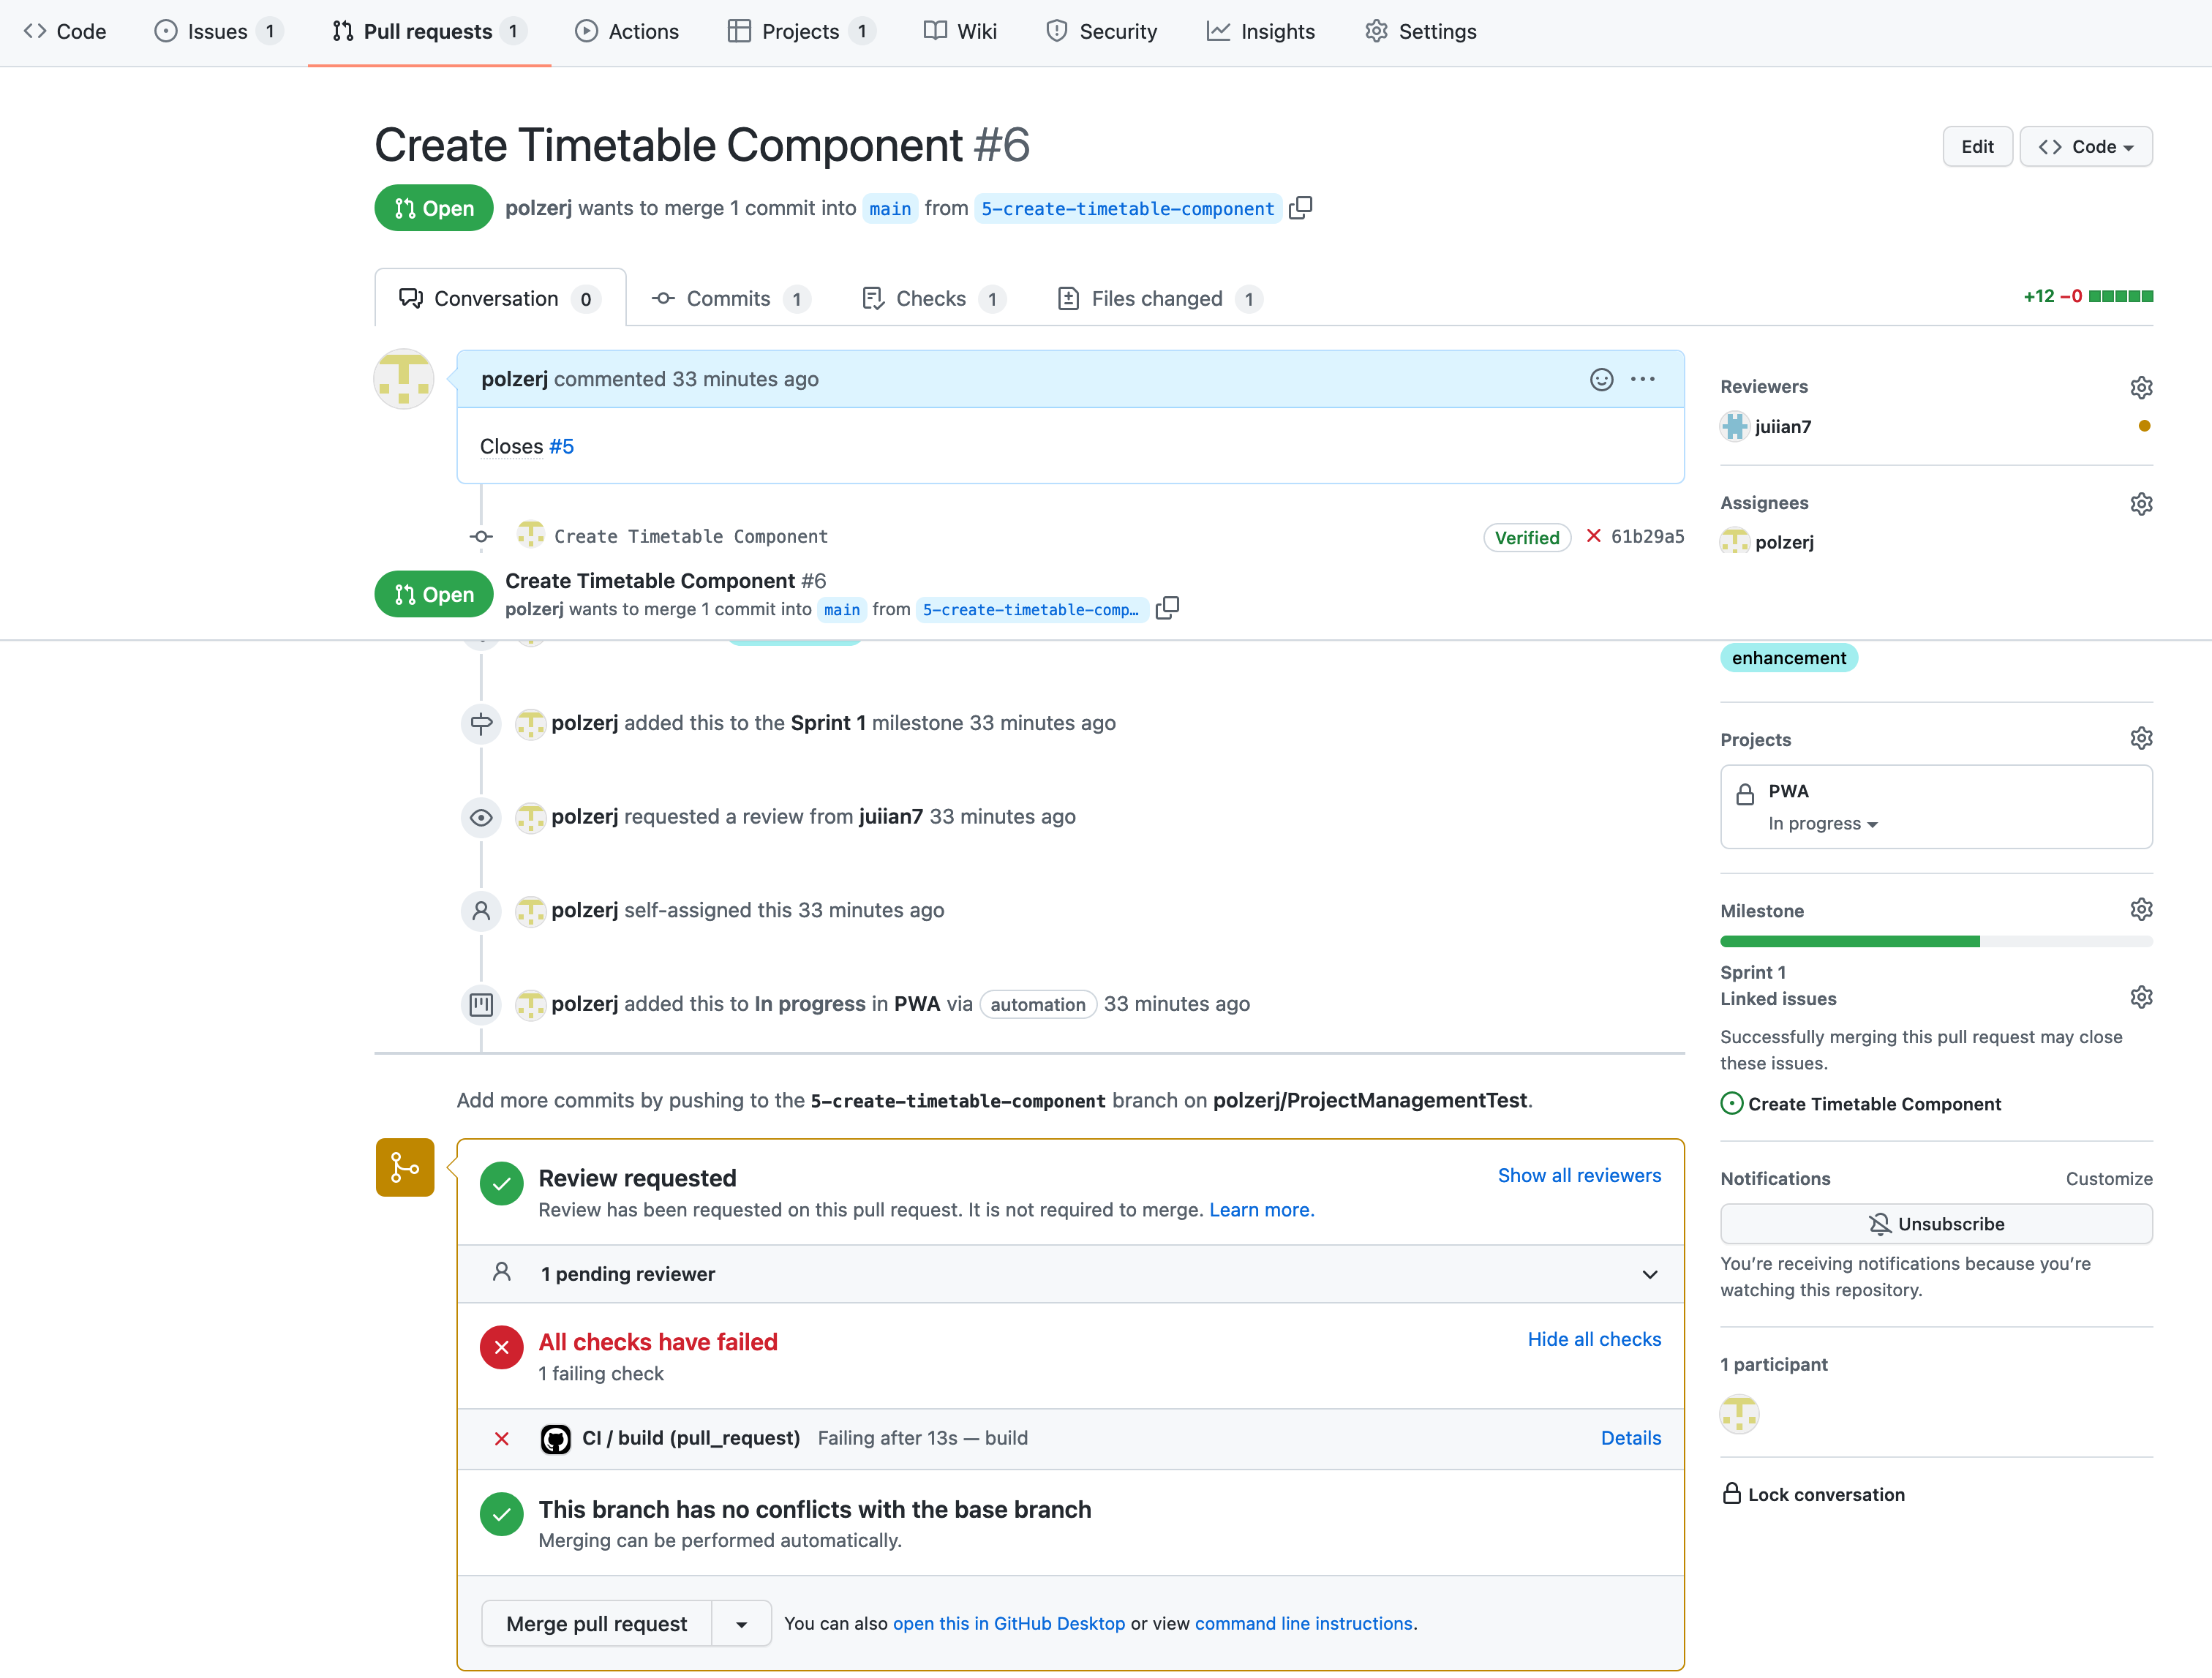
\includegraphics[width=\textwidth]{media/ProjectManagement/PullInfo.png}
    \caption{Detailansicht "Pull Requests" (Demo-Bild)}
    \label{fig:pullInfo}
\end{figure}

\hthree{Wiki}

In dem Wiki-Tab können Informationen über das Projekt abgelegt werden. Diese Seiten werden in Markdown geschrieben. Markdown bietet eine einfache Syntax, um Überschriften, Links, Listen, Code-Auszeichnungen und mehr zu erstellen. In der Seitenleiste kann zu Überschriften navigiert werden. (Siehe Abbildung \ref{fig:Projektantrag}) Allerdings kann diese Seitenleiste auch selber überschrieben werden.

\begin{figure}[H]
    \centering
    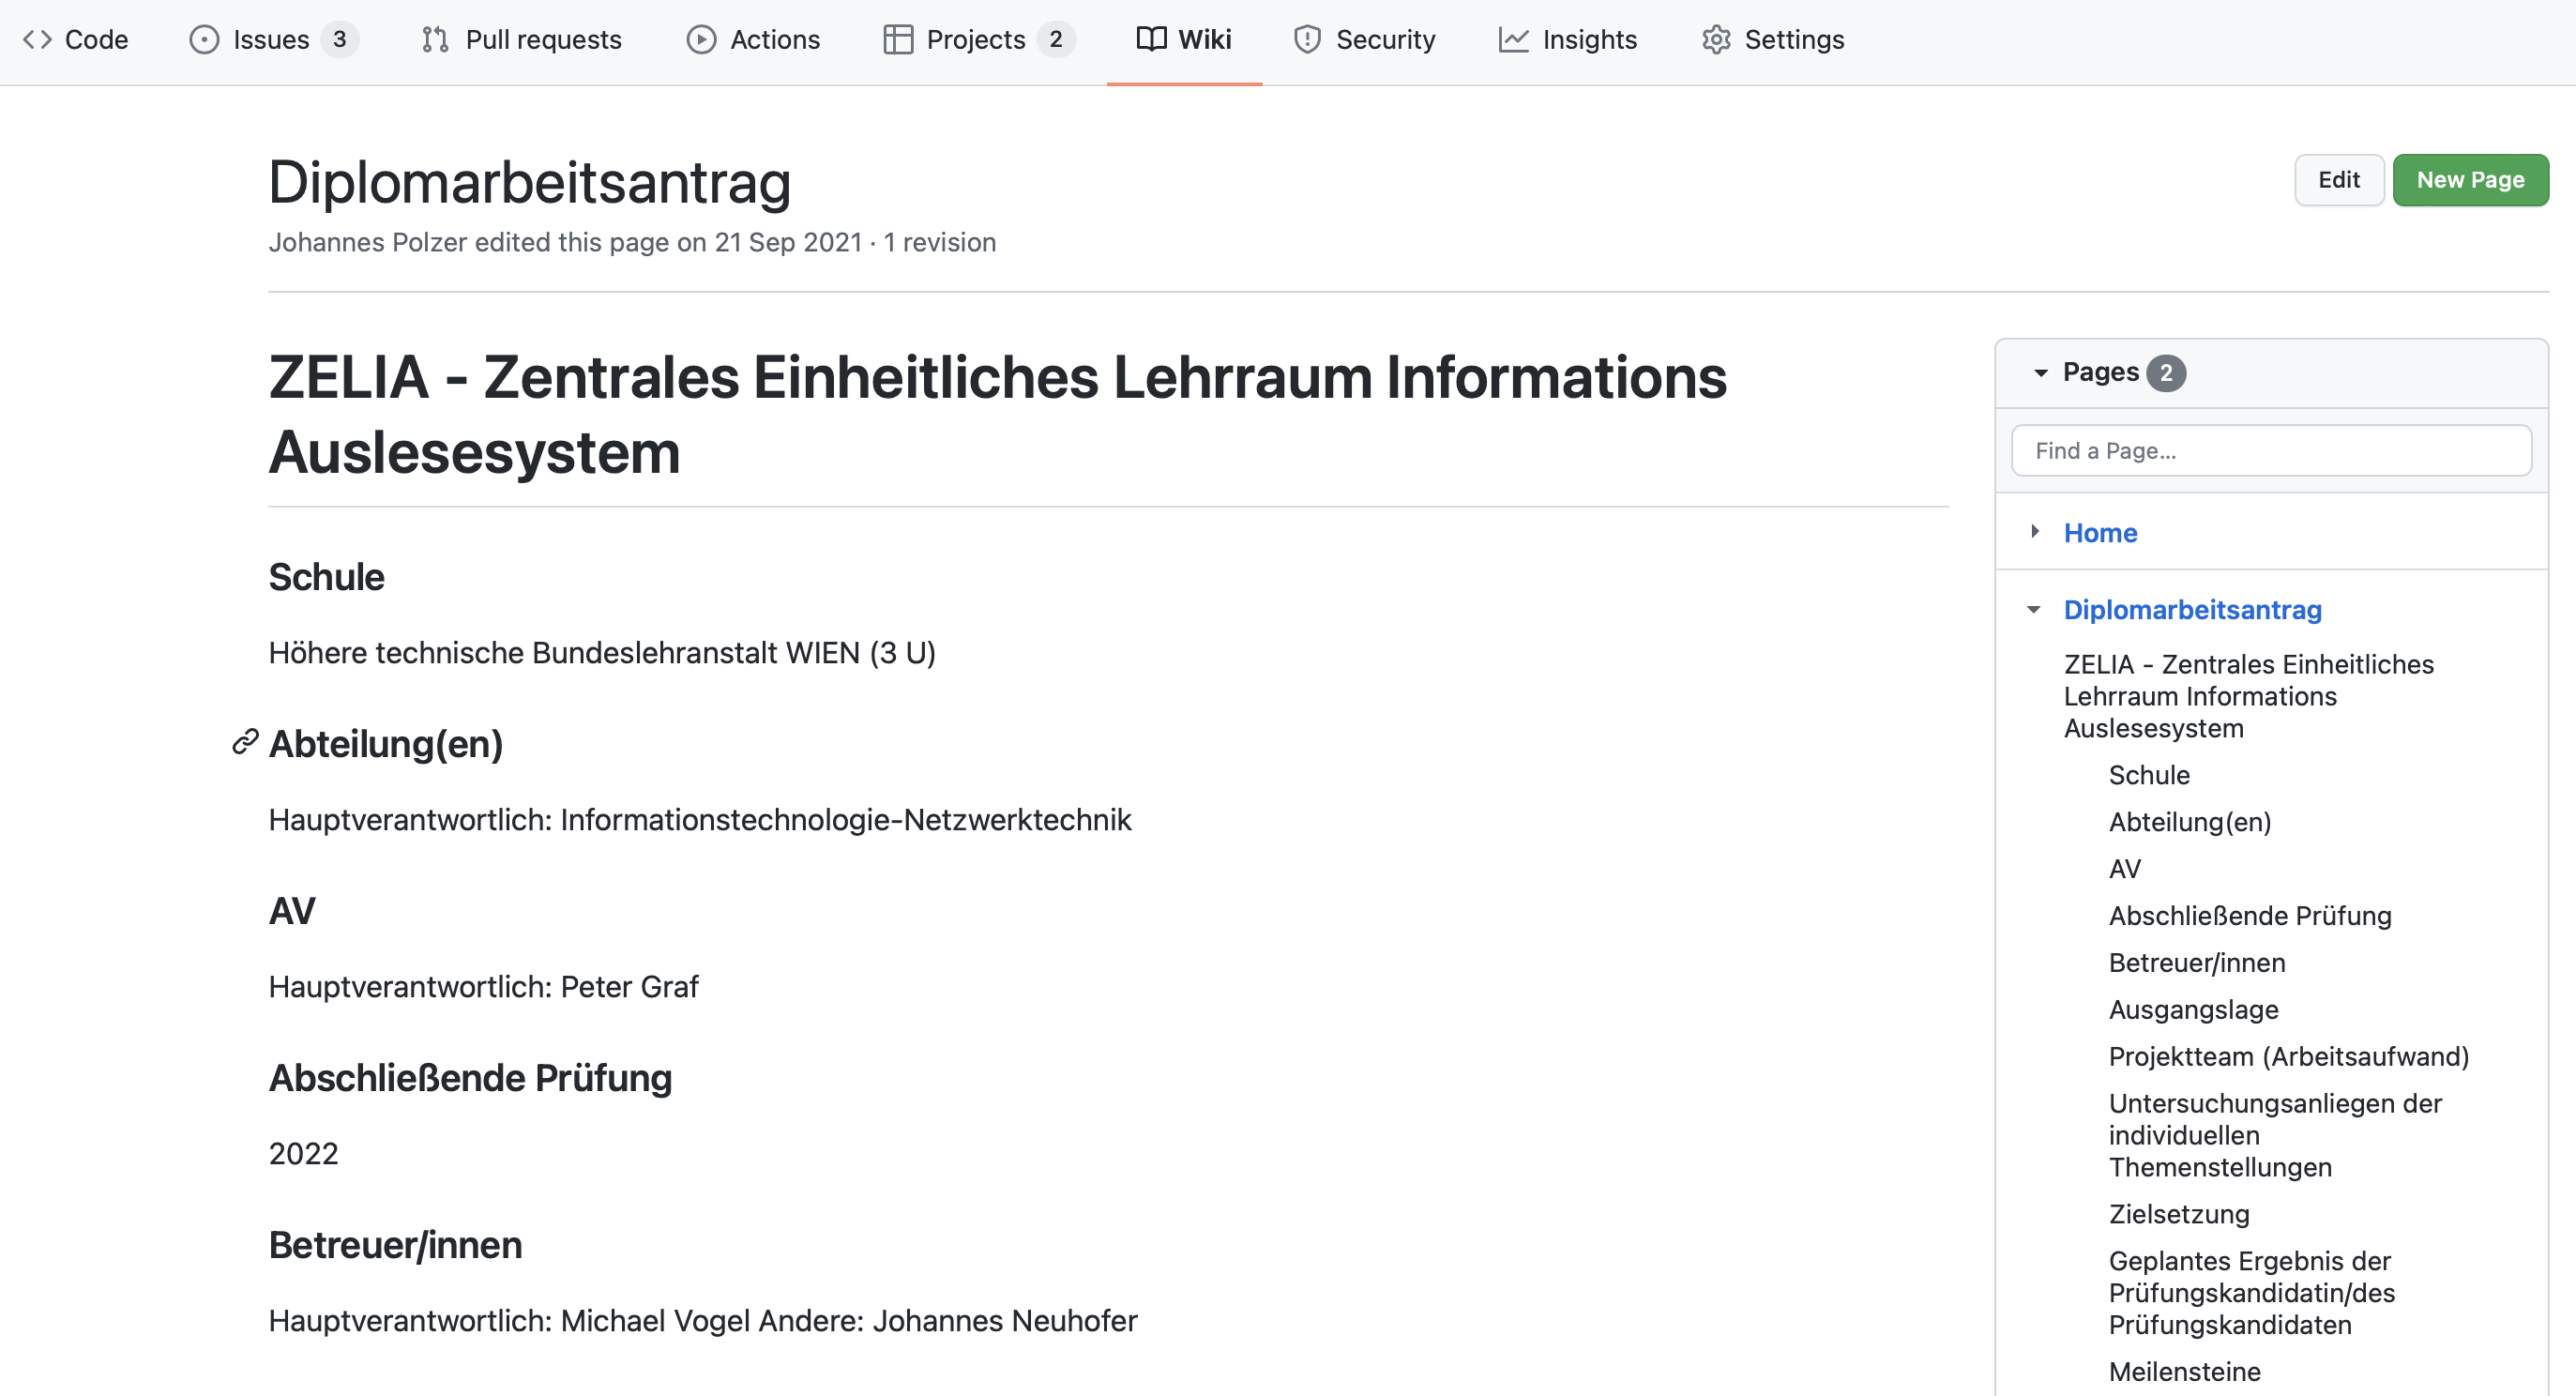
\includegraphics[width=\textwidth]{media/ProjectManagement/Wiki.png}
    \caption{Projektantrag in Github-Wiki}
    \label{fig:Projektantrag}
\end{figure}

Diese Seiten sind auch offline bearbeitbar. Dabei muss lediglich "wiki." vor "git" im Pfad des Repositories eingefügt werden, um das Wiki Repository zu clonen. Das heißt, aus {\ttfamily git@github.com:polzerj/Zelia.git} wird {\ttfamily git@github.com:polzerj/Zelia.wiki.git}. 

\hthree{Insights}

Die Insights ermöglichen es Statistiken über das Projekt auszulesen. Darin sind zum Beispiel die "Contributions" der einzelnen Personen aufgeführt. (Siehe Abbildung \ref{fig:insights})

\begin{figure}[H]
    \centering
    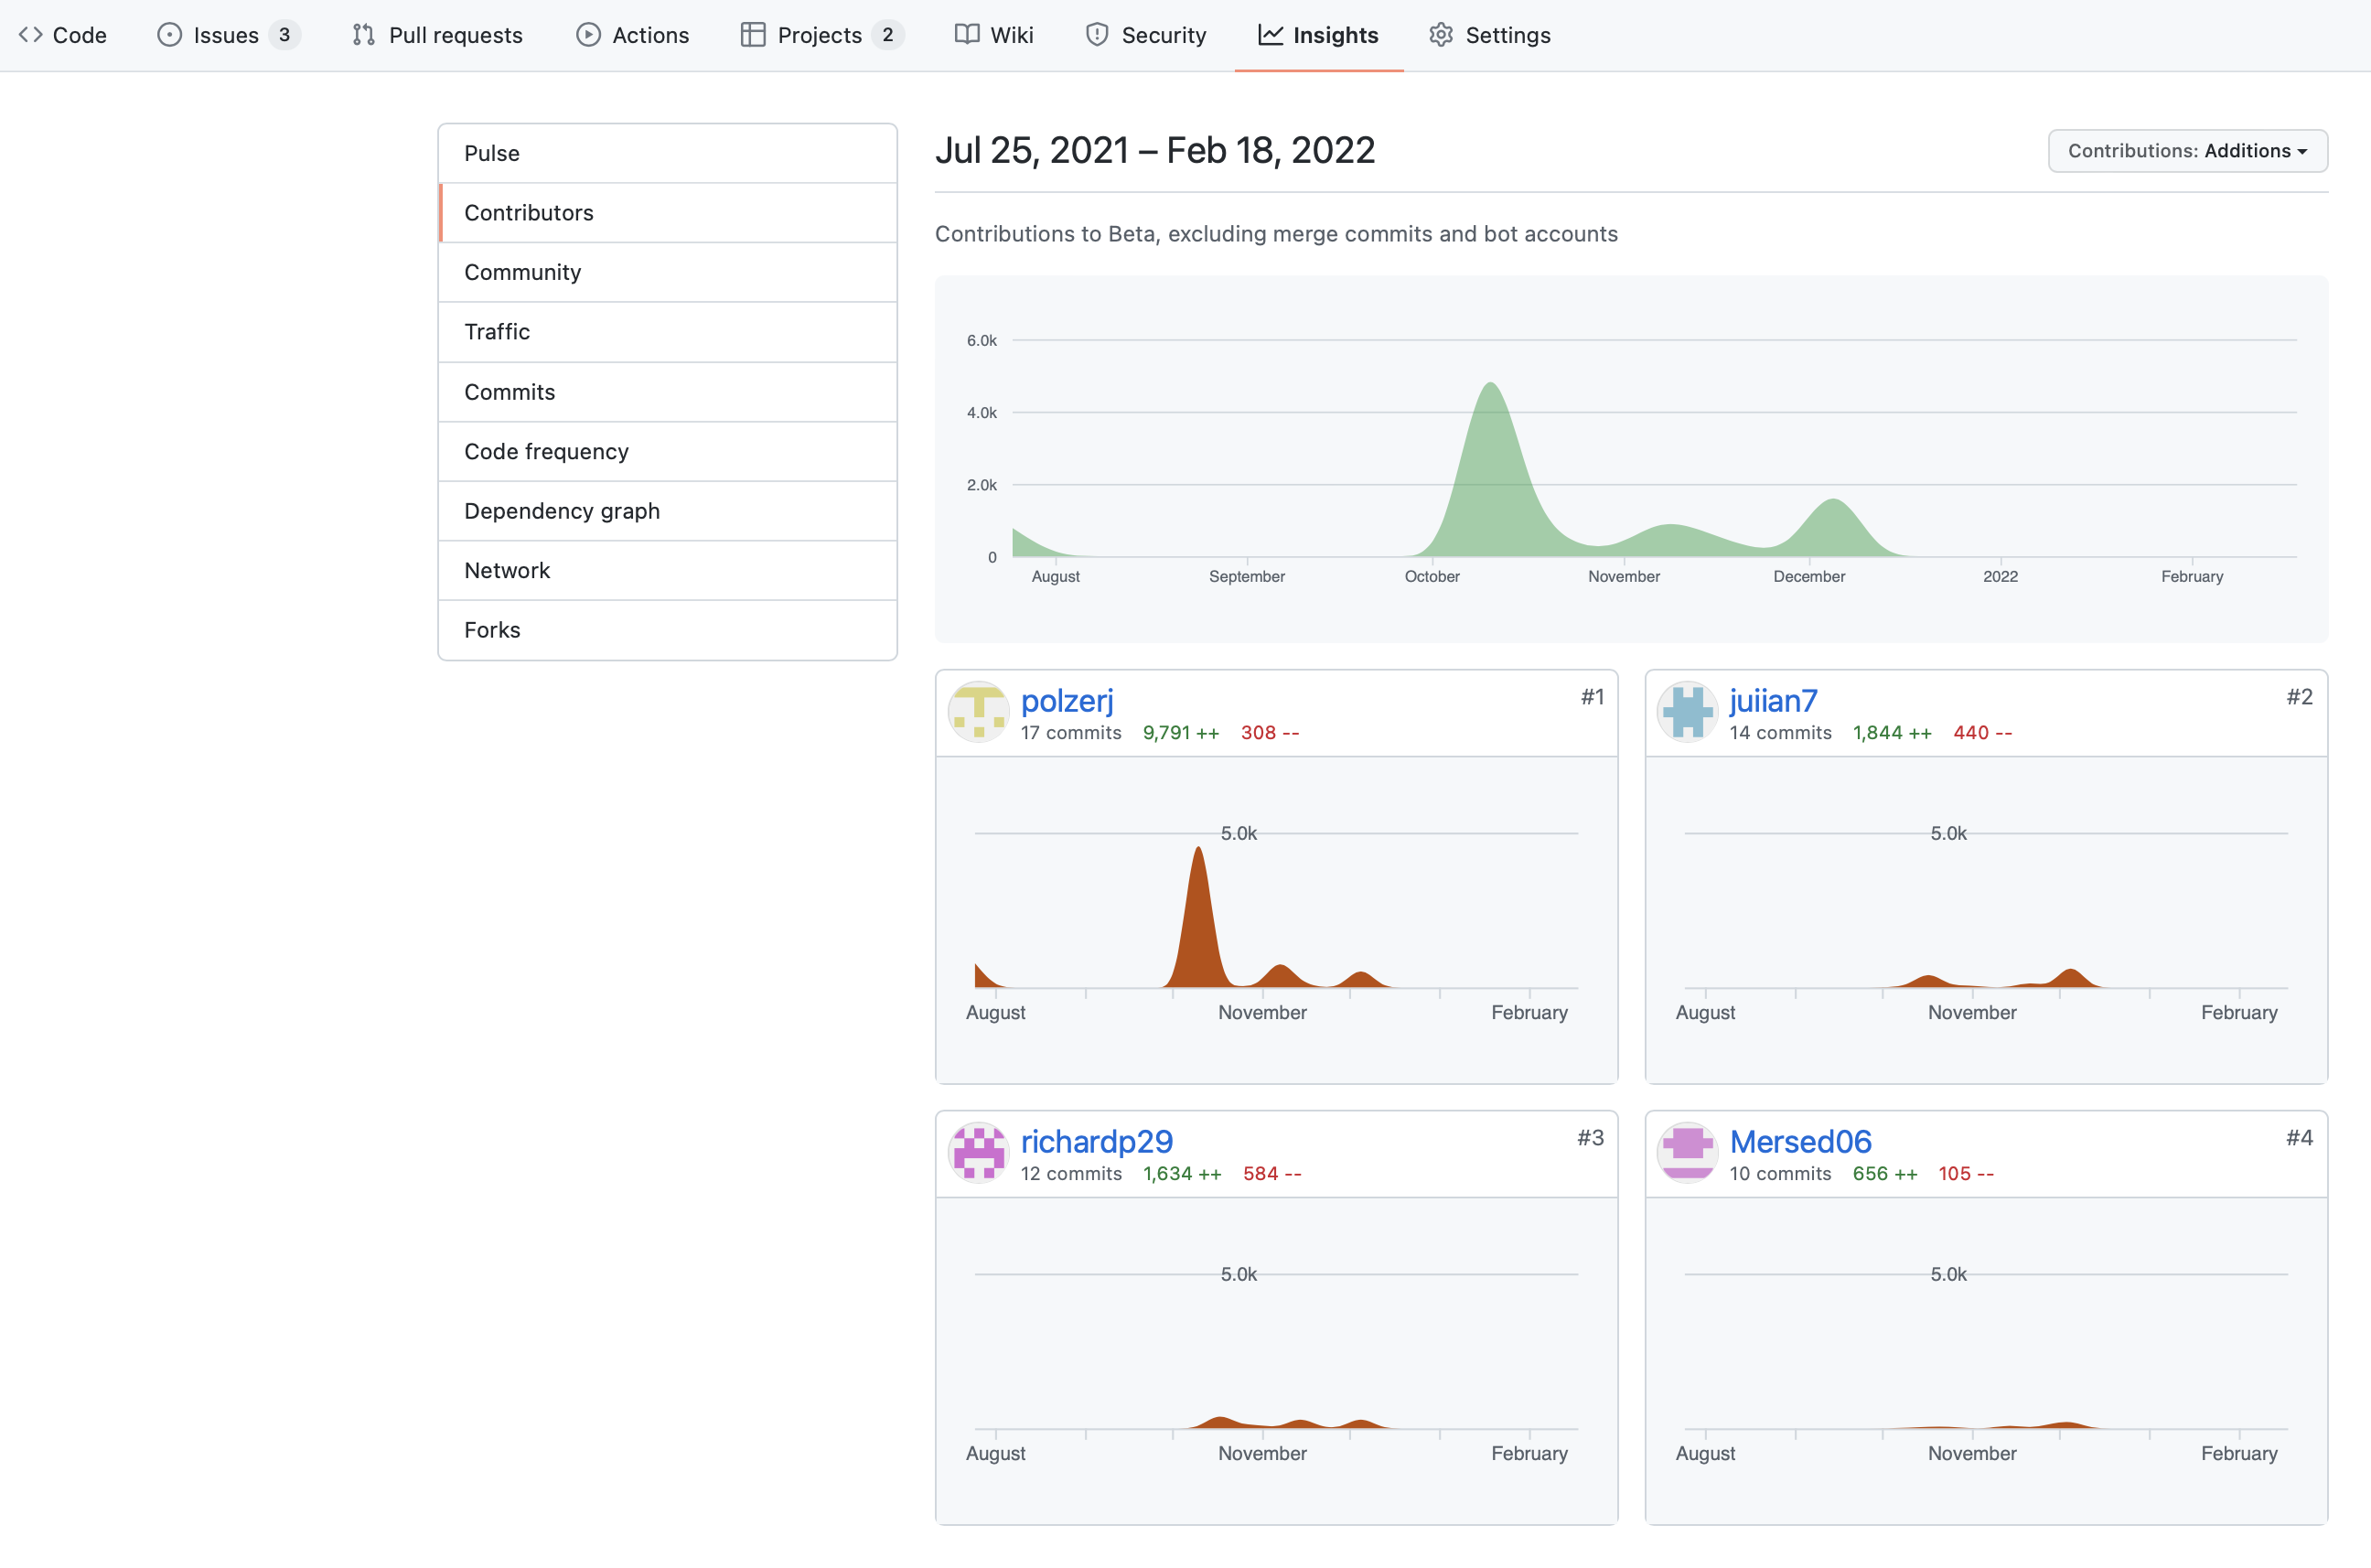
\includegraphics[width=\textwidth]{media/ProjectManagement/Insights.png}
    \caption{Statistik des Entwicklungsbeitrages der einzelnen Projektteilnehmer}
    \label{fig:insights}
\end{figure}